\chapter{Descrição técnica dos sistemas}
\label{descricao_tecnica_dos_sistemas}

\section{Resumo da Especificação de requisitos}
Com a aplicação da sistema ePadaria vai se promover e otimizar a comunicação e funcionamento dos 3 setores, pedidos, cozinha e entregas.\\
Na gestão de pedidos, o gestor de pedidos, só terá que preencher dados na aplicação ePadaria, esta que trata de comunicar e verificar o stock e também pedidos anteriores, que certifica que haverá espaço para o pedido no dia alocado, e dando ao gestor de pedidos imediatamente uma validação do pedido ou refere o que estava invalido no pedido.\\
Na gestão de pedidos, o gestor de pedidos, só terá que preencher dados na aplicação ePadaria, esta que trata de comunicar e verificar o stock e também pedidos anteriores, que certifica que haverá espaço para o pedido no dia alocado, e dando ao gestor de pedidos imediatamente uma validação do pedido ou refere o que estava invalido no pedido.\\


\section{Descrição do software que será necessário desenvolver}
\subsection{Requisitos funcionais}
\subsubsection{Casos de uso}
Na figura abaixo representa-se o modelo genérico de casos de uso do sistema ePadaria sob a forma de um diagrama de pacotes. Cada pacote agrega uma ou mais partes do sistema que se destinam a suportar processos da organização e/ou a reunir um conjunto de funcionalidades. Em cada pacote incluem-se alguns exemplos de Atores e casos de uso desenvolvidos para o sistema.

\begin{figure}[H]
	\centering
	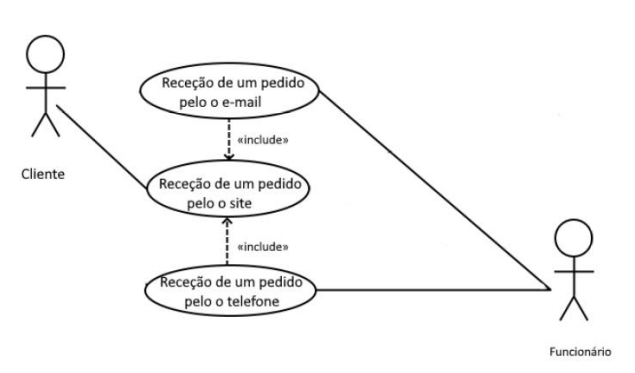
\includegraphics{diagrama_casos_de_uso}
	\caption{Diagrama de casos de uso}
	\label{fig:diagramacasosdeuso}
\end{figure}

\subsubsection{Requisitos}
Lista de requisitos para o caso de uso Receção de um pedido feito no site.\\
\begin{figure}[H]
	\centering
	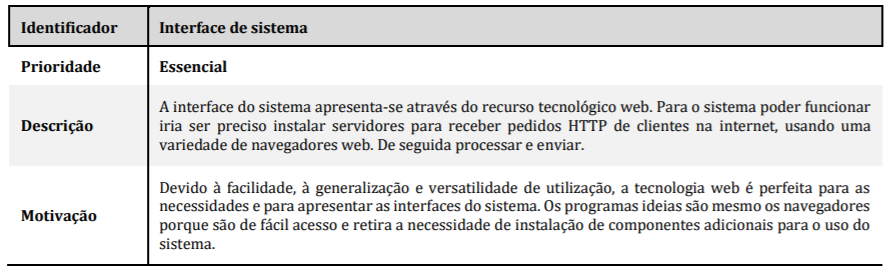
\includegraphics[width=15cm]{requisito_funcional1}
	\caption{Requisito funcional Interface do sistema}
	\label{fig:requisitofuncional1}
\end{figure}

\begin{figure}[H]
	\centering
	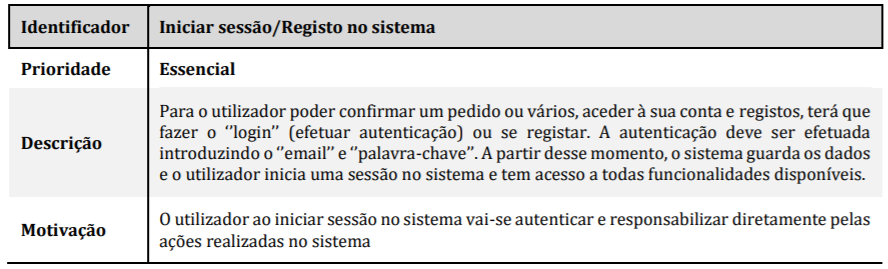
\includegraphics[width=15cm]{requisito_funcional2}
	\caption{Requisito funcional Iniciar Sessão/Registo no sistema}
	\label{fig:requisitofuncional2}
\end{figure}

\begin{figure}[H]
	\centering
	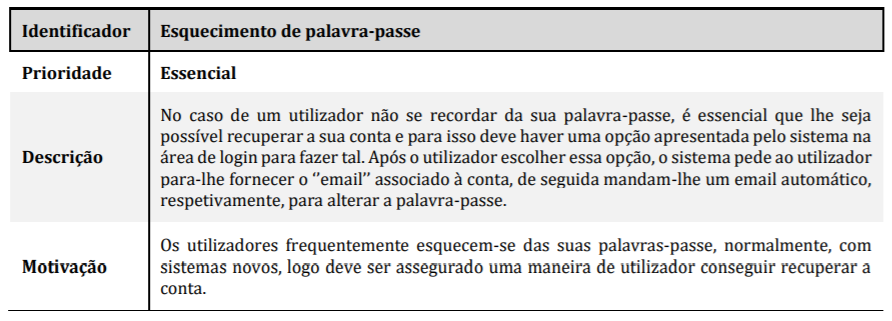
\includegraphics[width=15cm]{requisito_funcional3}
	\caption{Requisito funcional Esquecimento da palavra-passe}
	\label{fig:requisitofuncional3}
\end{figure}

\begin{figure}[H]
	\centering
	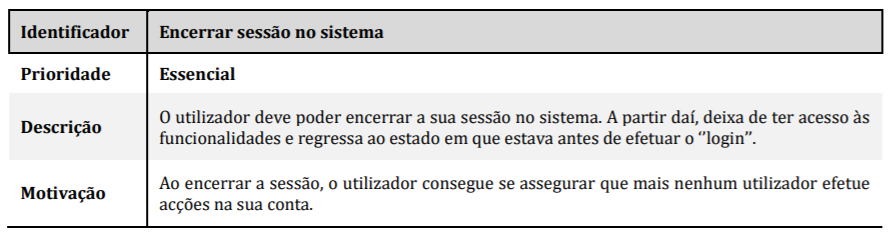
\includegraphics[width=15cm]{requisito_funcional4}
	\caption{Requisito funcional Encerrar sessão no sistema}
	\label{fig:requisitofuncional4}
\end{figure}

Lista de requisitos para o caso de uso Receção de um pedido efetuado por telefone.\\

\begin{figure}[H]
	\centering
	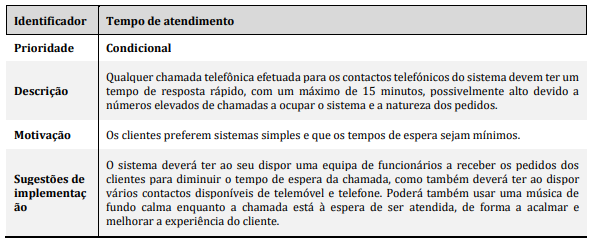
\includegraphics[width=15cm]{requisitofuncional5}
	\caption{Requisito funcional tempo de atendimento}
	\label{fig:requisitofuncional5}
\end{figure}

\begin{figure}[H]
	\centering
	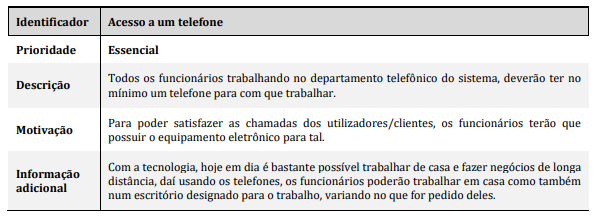
\includegraphics[width=15cm]{requisitofuncional6}
	\caption{Requisito funcional acesso a um telefone}
	\label{fig:requisitofuncional6}
\end{figure}



\begin{figure}[H]
	\centering
	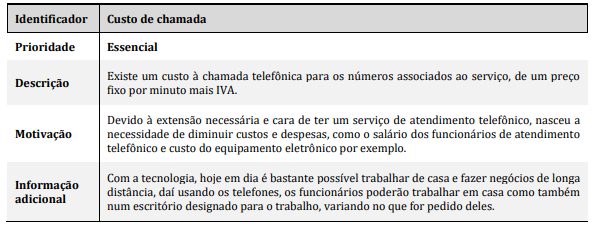
\includegraphics[width=15cm]{requisitofuncional7}
	\caption{Requisito funcional custo de chamada}
	\label{fig:requisitofuncional7}
\end{figure}

Lista de requisitos para o caso de uso Receção de um pedido efetuado por e-mail.\\

\begin{figure}[H]
	\centering
	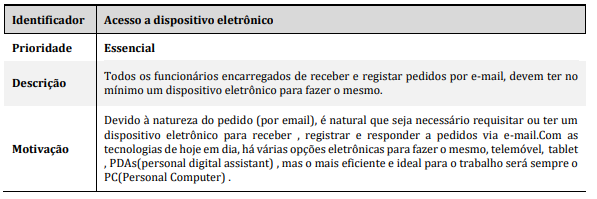
\includegraphics[width=15cm]{requisitofuncional8}
	\caption{Requisito funcional acesso a dispositivo eletrónico}
	\label{fig:requisitofuncional8}
\end{figure}

\subsubsection{Requisitos não-funcionais}

\begin{figure}[H]
	\centering
	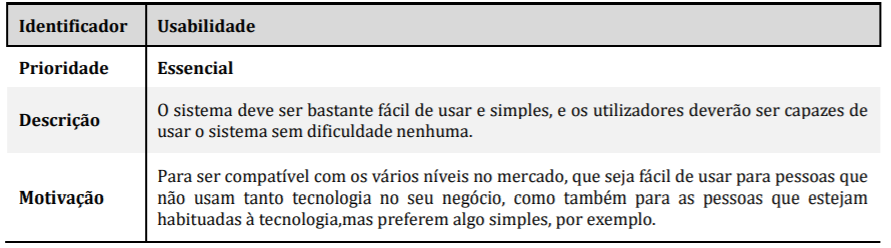
\includegraphics[width=15cm]{requisito_nao_funcional1}
	\caption{Requisito não funcional Usabilidade}
	\label{fig:requisitonaofuncional1}
\end{figure}

\begin{figure}[H]
	\centering
	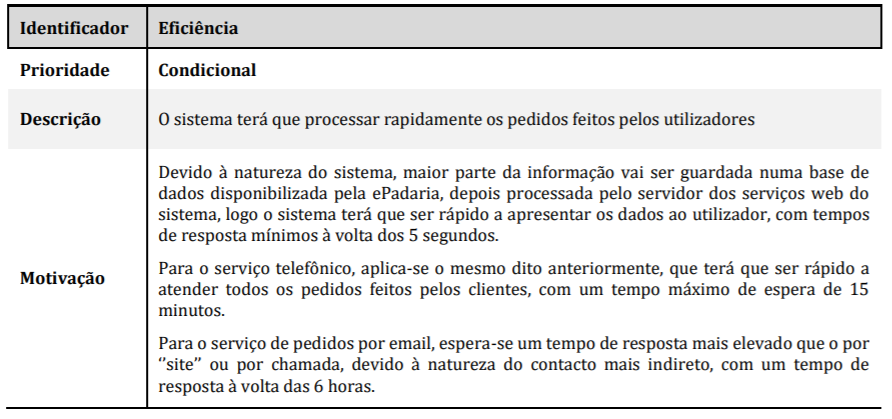
\includegraphics[width=15cm]{requisito_nao_funcional2}
	\caption{Requisito não funcional Eficiência}
	\label{fig:requisitonaofuncional2}
\end{figure}

\begin{figure}[H]
	\centering
	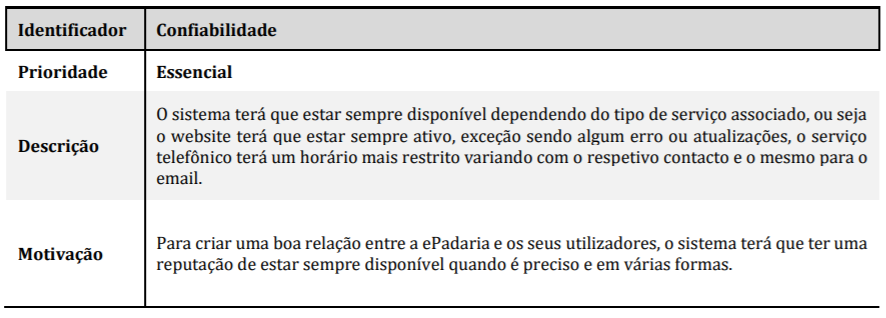
\includegraphics[width=15cm]{requisito_nao_funcional3}
	\caption{Requisito não funcional Confiabilidade}
	\label{fig:requisitonaofuncional3}
\end{figure}

\begin{figure}[H]
	\centering
	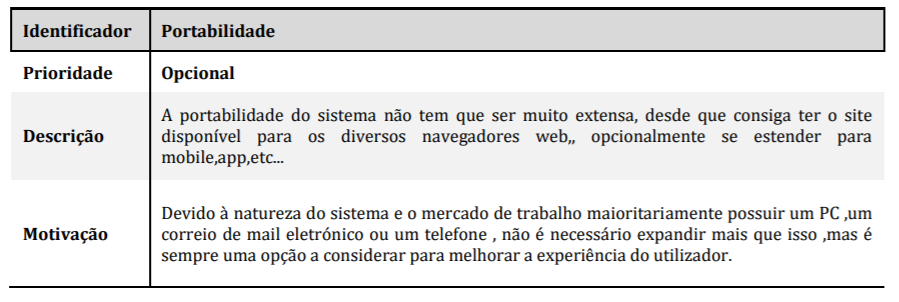
\includegraphics[width=15cm]{requisito_nao_funcional4}
	\caption{Requisito não funcional Portabilidade}
	\label{fig:requisitonaofuncional4}
\end{figure}

\begin{figure}[H]
	\centering
	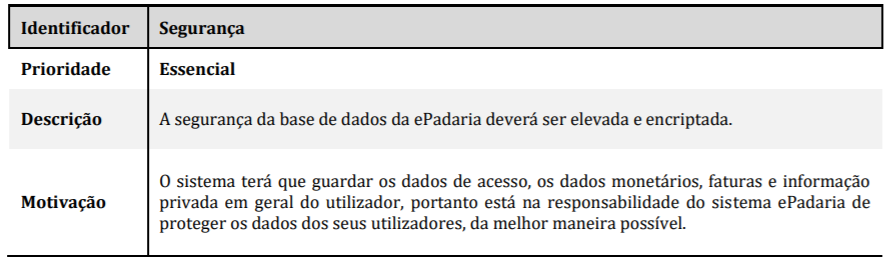
\includegraphics[width=15cm]{requisito_nao_funcional5}
	\caption{Requisito não funcional Segurança}
	\label{fig:requisitonaofuncional5}
\end{figure}

\begin{figure}[H]
	\centering
	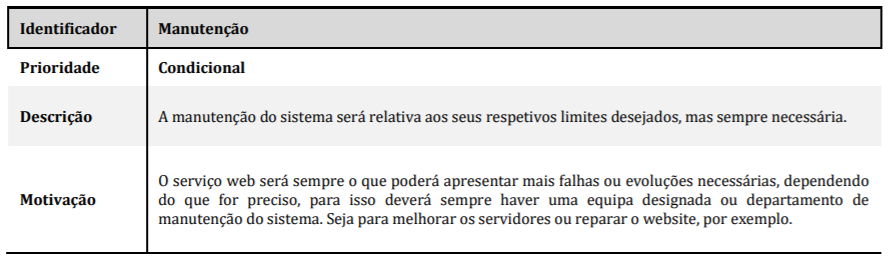
\includegraphics[width=15cm]{requisito_nao_funcional6}
	\caption{Requisito não funcional Manutenção}
	\label{fig:requisitonaofuncional6}
\end{figure}

\section{Descrição do estrutura física do hardware}
A maneira mais viável de efeituar o seu uso, seria num computador ou tablet, porque devido á estrutura mais pequena do telemóvel é mais difícil de usar, logo foi desenhado mais para uso no computador e nos seus "browsers". \\
Não é necessário ter um dispositivo de alto desempenho para se poder aceder ao site e ser usado, apenas é necessário ter os requisitos mínimos.\\
De acordo com um documento de \textbf{Requisitos de aplicação Web da Microsoft}, os \textbf{requisitos mínimos e recomendados de hardware} são:\\
\\ \textbf{Mínimo}\\
\\Processador - Processador dual core x86 ou x64 bits de 1,9 gigahertz (GHz) com conjunto de instruções SSE2.\\
\\Memória - 2 GB de RAM. \\
\\Monitor - Super VGA com uma resolução de 1024 x 768. \\
\\ \textbf{Recomendado}\\
\\Processador - Processador dual core 64 bits de 3,3 gigahertz (GHz) ou mais rápido com conjunto de instruções SSE2.\\
\\Memória - 4 GB de RAM ou mais.\\
\\Monitor - 	Super VGA com uma resolução de 1024 x 768.\\
\\"A execução de aplicações condicionadas por modelos num computador com uma configuração inferior aos requisitos recomendados pode originar um desempenho inadequado. Além disso, poderá verificar-se um desempenho satisfatório na execução de sistemas que utiliza, uma configuração de hardware diferente da aqui publicada, por exemplo, um sistema de com um processador quad-core moderno, velocidade de relógio inferior e mais RAM."\\
\\Os \textbf{requisitos de rede} não são muito pesados devido á natureza do sistema, mas é recomendado na mesma no mínimo :\\
\\- Mais de 50 kbps (400 kbps) de largura de banda\\
\\- Latência abaixo de 150 ms\\
\\Por parte dos funcionários da padaria o melhor é usar algo e pelo menos médio desempenho de maneira a o sistema responder de forma rápida e não atrasar a produtividade.\\

\begin{figure}[H]
	\centering
	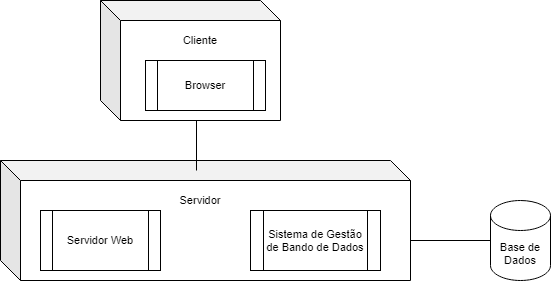
\includegraphics[width=15cm]{Diagarama_Dist}
	\caption{Diagrama de distribuição}
	\label{fig:Diagarama_Dist}
\end{figure}


\section{Descrição da interface gráfica}

A interface gráfica da ePadaria tem em conta a usabilidade e o necessário para atender as expectativas visuais dos nossos clientes e dos clientes das padarias. Em qualquer parte do site será possível aceder à página inicial, aos contactos, “sobre nós" onde se encontra informação sobre o ePadaria, apenas não será possível aceder a essas páginas pela página do funcionário.
\begin{figure}[H]
	\centering
	\includegraphics[width=15cm]{"mockup sobre nos"}
	\caption{Página Web da ePadaria: Sobre nós}
	\label{fig:mockup-sobre-nos}
\end{figure}

\begin{figure}[H]
	\centering
	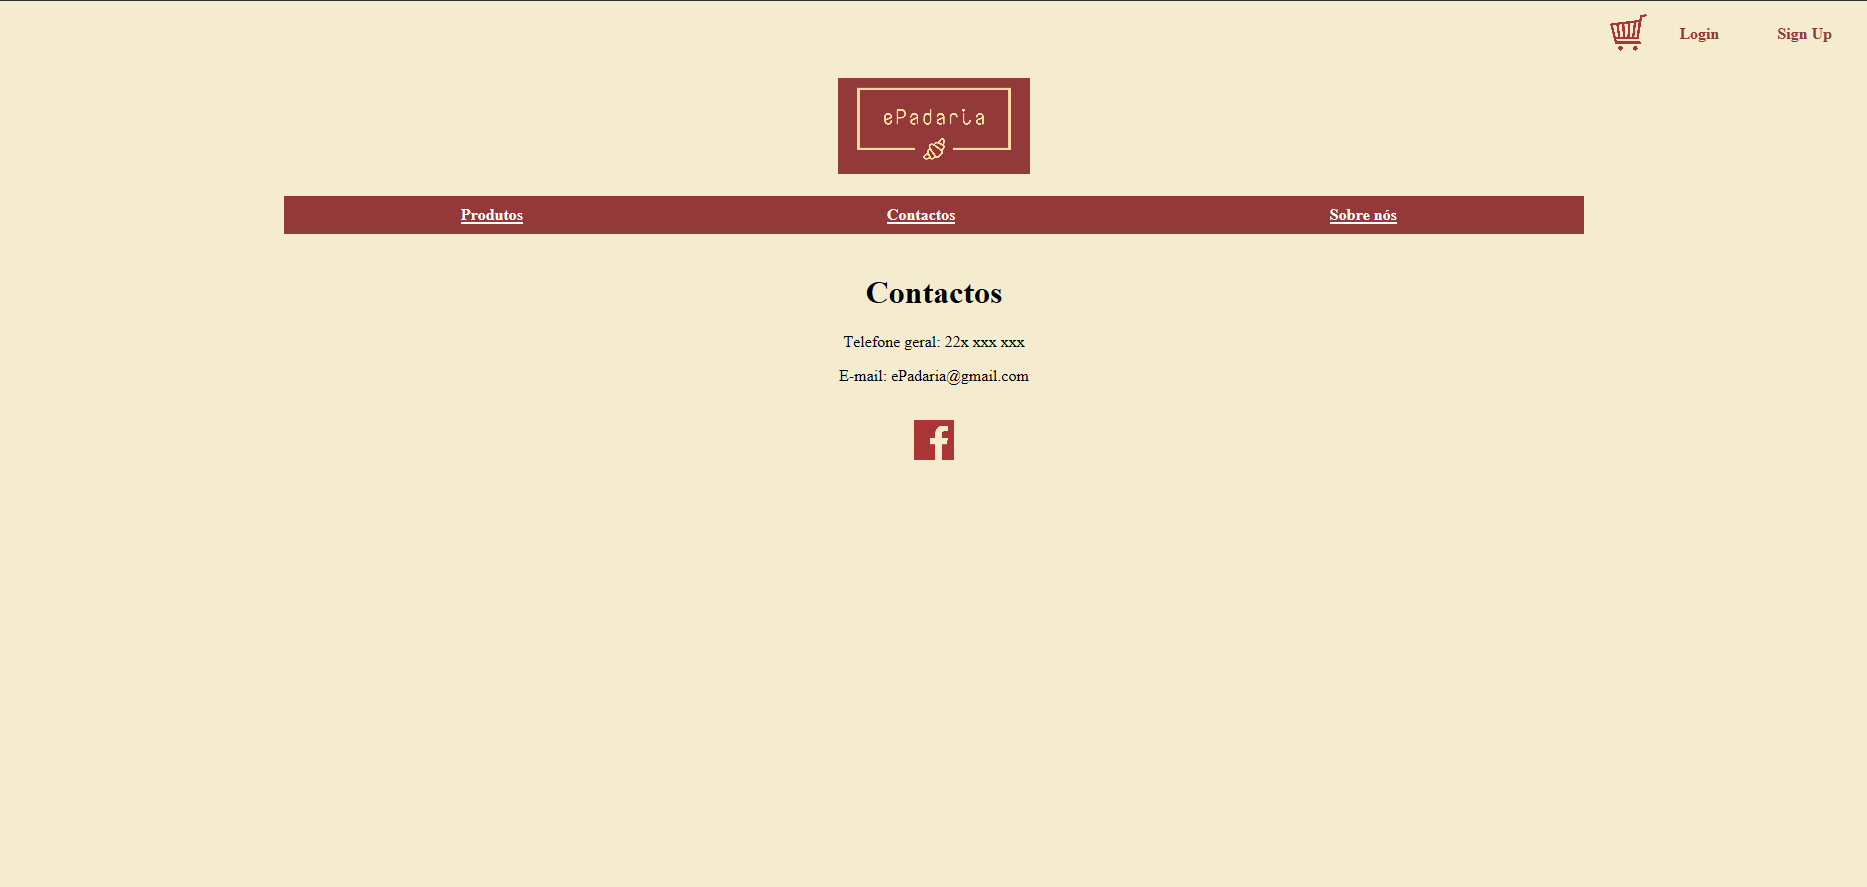
\includegraphics[width=15cm]{Contactos}
	\caption{Página Web da ePadaria: Contactos}
	\label{fig:Contactos}
\end{figure}

\begin{figure}[H]
	\centering
	\includegraphics[width=15cm]{Produtos1}
	\caption{Página Web da ePadaria: Mensagem de aviso}
	\label{fig:produtos1}
\end{figure}

Se um utilizador carregar em produtos ou no carrinho sem estar "logged in", aparece esta mensagem de aviso/erro para procederem a fazer o "login" ou "sign up".

\begin{figure}[H]
	\centering
	\includegraphics[width=15cm]{"mockup sig in"}
	\caption{Página Web da ePadaria: Sign Up}
	\label{fig:mockup-sig-in}
\end{figure}

O sistema "sign up" que definimos com os campos que tem de ser preenchidos e de seguida, estes mesmos dados entram na nossa base de dados e os clientes ficam registados.

\begin{figure}[H]
	\centering
	\includegraphics[width=15cm]{"mockup log in"}
	\caption{Página Web da ePadaria: Log in}
	\label{fig:mockup-log-in}
\end{figure}

Após efetuar o "login", o ícone "Login"  irá aparecer com o nome do cliente que definiu no site.\\
Se o funcionário quiser entrar na página definida para si, terá que aceder ao "login"  e de seguida escolher a opção  "LogIn Funcionário".

\begin{figure}[H]
	\centering
	\includegraphics[width=15cm]{"mockup page func"}
	\caption{Página Web da ePadaria: Página do funcionário}
	\label{fig:mockup-page-func}
\end{figure}

De seguida irá aparecer uma mensagem com o nome do funcionário após o "Bem-vindo".\\
Aqui o funcionário vai ter a opção de mexer no stock registado na base de dados, podendo assim gerir o sistema de maneira fácil e simples.
O funcionário também vai poder mexer com os pedidos, podendo registar os feitos e realizados, os que estão á espera de ser entregues e o histórico dos mesmos.\\

\begin{figure}[H]
	\centering
	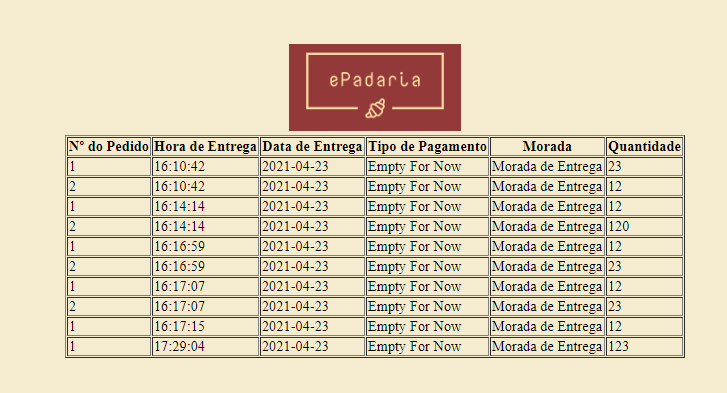
\includegraphics[width=15cm]{produtos33}
	\caption{Página Web da ePadaria: Histórico de pedidos }
	\label{fig:produtos33}
\end{figure}
Após efetuar o login de funcionário, ele mesmo poderá aceder ao histórico de pedidos feitos na sua padaria para a gerir.

\begin{figure}[H]
	\centering
	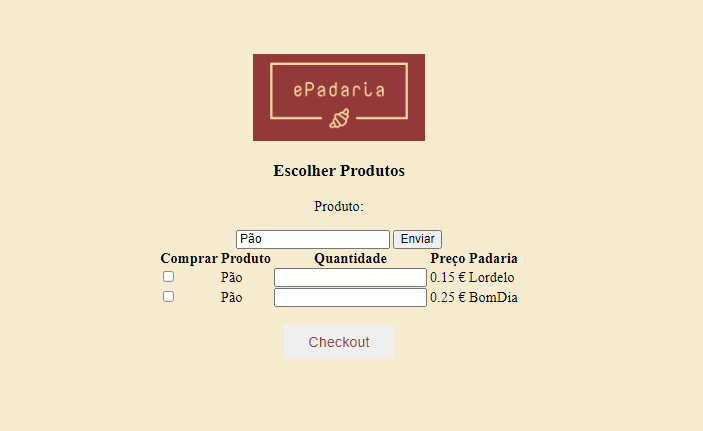
\includegraphics[width=15cm]{produtos2}
	\caption{Página Web da ePadaria: Carrinho/Comprar}
	\label{fig:produtos2}
\end{figure}
Nesta imagem temos um mock-up muito inicial do carrinho após o "login" e ter carregado no cesto/carrinho de compras.